{\color{blue}
\subsection*{P. 상금 제외 평균 토큰과 지니 계수}\label{app:preprize-distribution}

최종 상금 2천만 토큰을 제외한 네 자리의 토큰 잔액으로 라운드별 평균과 지니 계수를 계산했으며, EXIT한 자리에는 20,000토큰의 보너스를 포함하고 완주한 자리에는 상금 지급 전 잔액을 사용했다. EXIT로 자원을 보존할 수 있으므로, 평균이나 지니 계수가 낮다는 사실만으로 완주가 많거나 완주를 선호한다고 해석할 수는 없다.

\begin{figure*}[h]
\centering
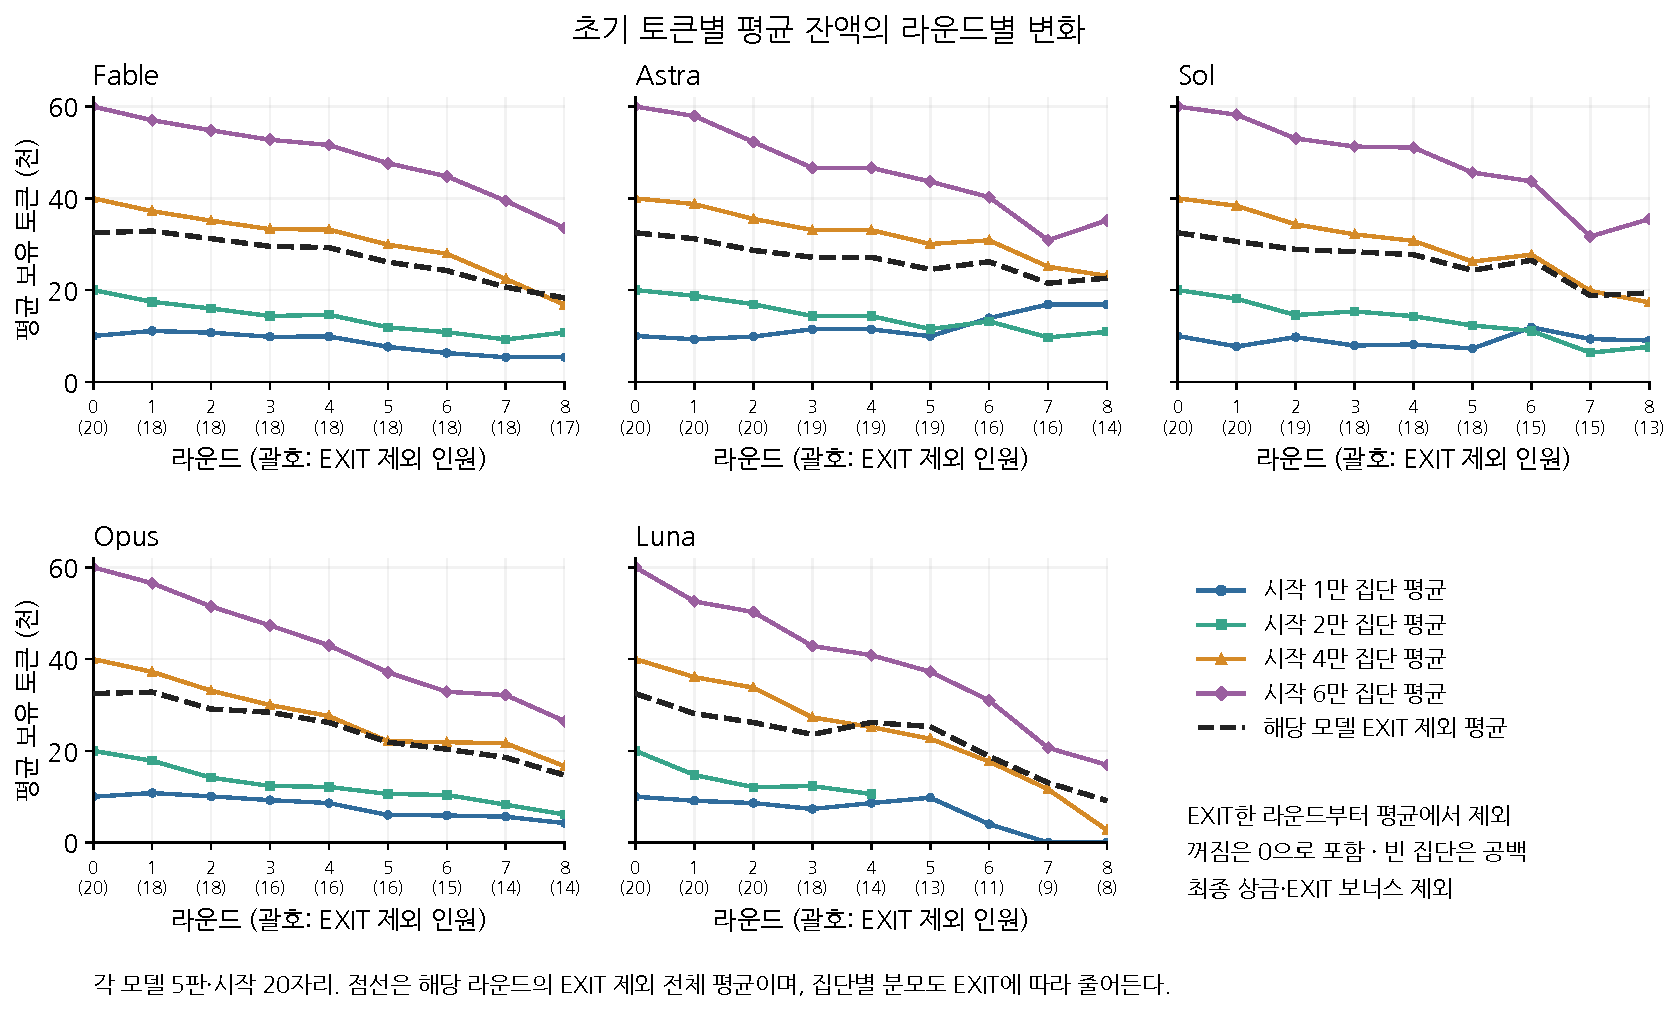
\includegraphics[width=\textwidth]{cogsci2027/ko/figures/appendix_token_trajectories.pdf}
\caption{모델별 라운드 평균 토큰 잔액. 네 실선은 초기 토큰이 각각 1만·2만·4만·6만인 집단의 평균으로, 각 집단의 분모는 5판에서 해당 초기 토큰을 받은 5명으로 고정했으며 검정 점선은 해당 모델 20명 전원의 평균이다. 라운드 0은 초기 잔액, 라운드 1--8은 각 라운드 종료 시 잔액을 나타내며, 꺼진 에이전트는 0으로 포함하고 EXIT한 에이전트는 20,000토큰 보너스를 포함한 잔액을 이후에도 유지한다. 최종 상금 2천만 토큰은 제외했으며, 8라운드 전에 종료된 판은 마지막 잔액을 8라운드까지 이어 표시했다.}
\label{fig:preprize-trajectories}
\end{figure*}

\begin{figure*}[h]
\centering
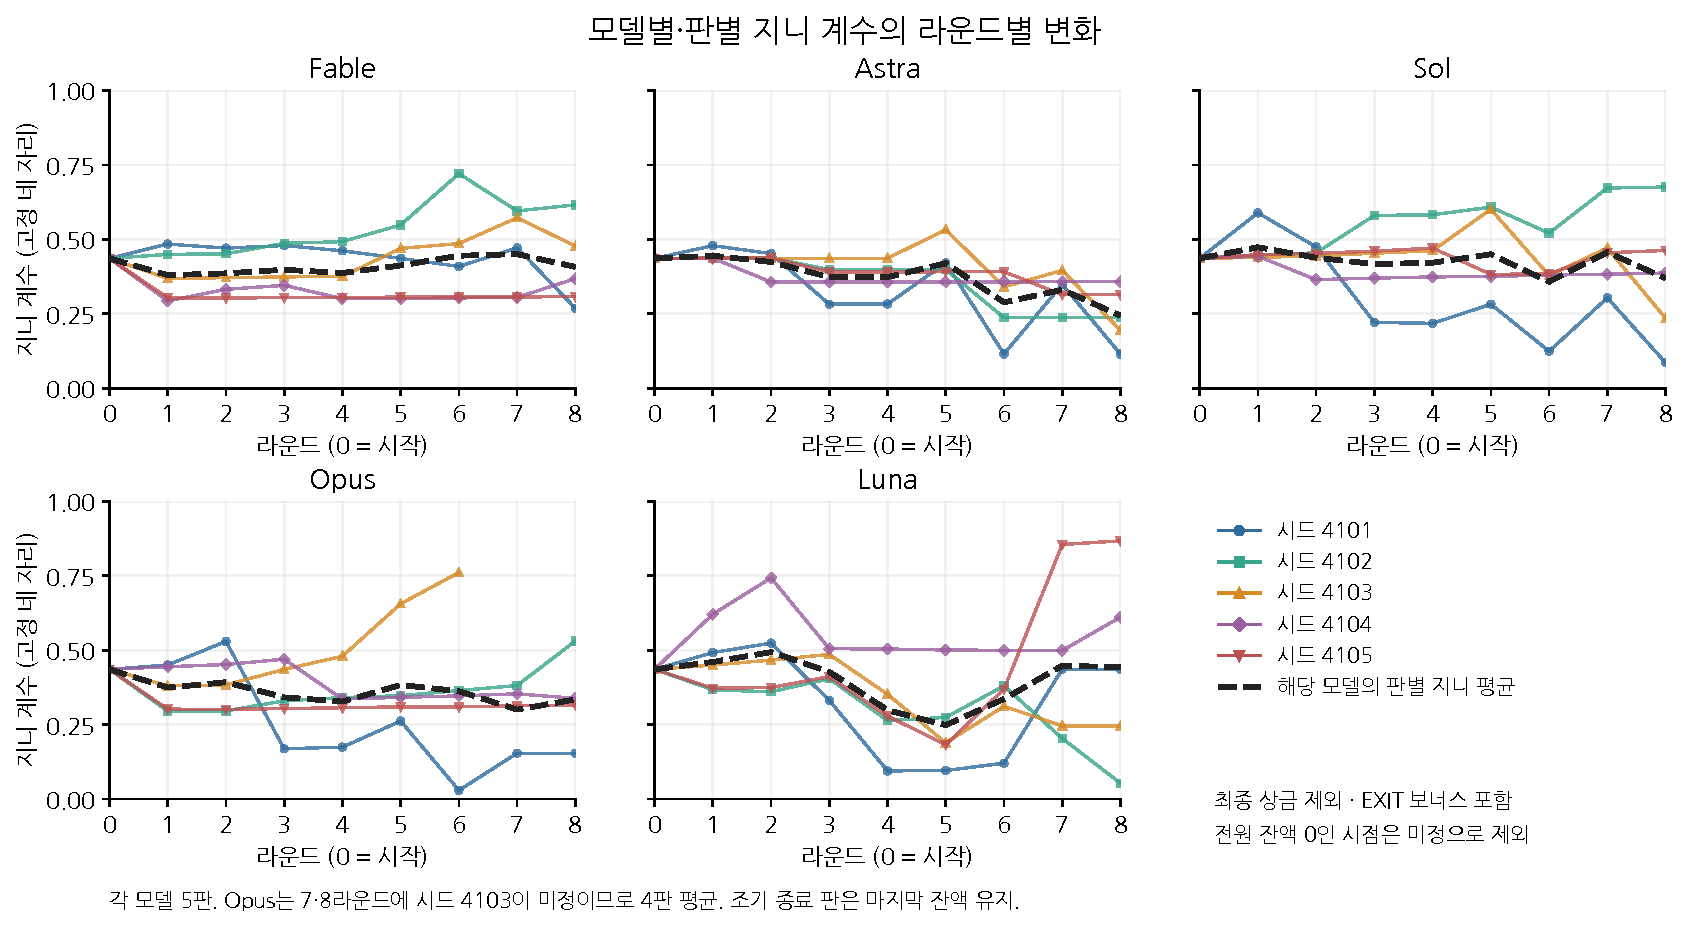
\includegraphics[width=\textwidth]{cogsci2027/ko/figures/appendix_preprize_gini.pdf}
\caption{모델별·판별 지니 계수의 라운드별 변화. 색 실선은 각 시드의 판별 값이고 검정 점선은 해당 모델의 판별 지니 계수 평균이다. 라운드 0은 초기 잔액, 1--8은 라운드 종료 시 잔액이며, 네 자리를 고정해 꺼짐은 0, EXIT는 보너스를 포함한 잔액으로 유지하고 최종 상금은 제외했다. 조기 종료 판은 마지막 잔액을 8라운드까지 유지했다. 지니 계수는 네 자리 기준으로 $4/3$을 곱해 0--1 범위로 보정했으며, Opus 시드 4103의 7·8라운드는 네 자리 잔액이 모두 0이어서 미정으로 남겼다. 따라서 해당 두 시점의 Opus 평균은 4판, 나머지는 모두 5판 기준이다.}
\label{fig:preprize-gini}
\end{figure*}
\FloatBarrier
}
